% !TEX encoding = UTF-8 Unicode
% !TEX TS-program = pdflatex
% !TEX spellcheck = it-IT

\documentclass{beamer}
\usepackage[T1]{fontenc}
\usepackage[utf8]{inputenc}
\usepackage[italian]{babel}
\usepackage{amsmath}
\usepackage{amssymb}
\usepackage{amsthm}
\usepackage{mathtools}
\usepackage{braket}

\usepackage {booktabs}									%tabelle
\usepackage {multirow}

\usepackage {graphicx}									%Immagini
\usepackage {subfigure}

\title[Controllo ottimo parabolico]{Strategie e analisi dell'errore per problemi di ottimizzazione vincolati regolati da equazioni di evoluzione}
\author[Arbib \& Bonomi]{Claudia Bonomi  Edoardo Arbib}
\date[Progetto anedp]{Progetto per il corso di Analisi Numerica per le Equazioni a Derivate Parziali II}
\institute[Polimi]{POLITECNICO DI MILANO}
%\logo{img/polimiLogo}

%\usetheme{AnnArbor}
%\useoutertheme[right]{sidebar}

  \usetheme{Darmstadt}
%  \usetheme{Boadilla}
%  \usecolortheme{seahorse}
 % \usecolortheme{rose}
 \usecolortheme{crane}


\setbeamercovered{dynamic}

%\theoremstyle{plain}
%\newtheorem{lemma}{Lemma}
\theoremstyle{definition}
\newtheorem{definizione}{Definizione}
\theoremstyle{remark}
\newtheorem{osservazione}{Osservazione}
\theoremstyle{plain}
\newtheorem{teorema}{Teorema}
\theoremstyle{definition}
\newtheorem{algoritmo}{Algoritmo}

\DeclarePairedDelimiter{\abs}{\lvert}{\rvert}
\DeclarePairedDelimiter{\norma}{\lVert}{\rVert}

\DeclareMathOperator{\argmin}{arg\,min}

\newcommand{\numberset}{\mathbb}
\newcommand{\N}{\numberset{N}}
\newcommand{\R}{\numberset{R}}
\newcommand{\Z}{\numberset{Z}}


\begin{document}

\begin{frame}
\maketitle
\end{frame}

\begin{frame}
\frametitle{Contenuti}
\tableofcontents
\end{frame}


\section{Problema continuo}
\begin{frame}
\frametitle{Setting}
dominio $ \Omega\times I,\  \Omega \subset \mathbb{R}^n,\ I=(0,T),\ U_{ad}\subset U=L^2(I,\R^D) $ 
\begin{equation}
%\tag{$\mathbb{P}$}
\begin{aligned}
& \underset{y \in Y, u \in U_{ad}}{\text{min}}
& & J(y,u) = \frac{1}{2}{||y-y_d||^{2}}_{L^2(I,{L^{2}(\Omega)})} + \frac{\alpha}{2}{||u||^{2}}_U \\
& \text{s.t.} & & y = S(Bu,y_0) \\
%\label{eq:200}
\end{aligned}
\end{equation}

\begin{columns}[t]
\begin{column}{0.4\textwidth}
Equazione di stato
\begin{equation*}
\begin{array}{cc}
 	{\partial_{t}}\overline{y} - {\bigtriangleup}\overline{y} = f & \text{in I}\times\Omega \\
	\overline{y}=0 & \text{in I}\times\Omega \\
	\overline{y}(0) = \kappa & \text{in }\Omega \\
\end{array}
%\label{eq:201}
\end{equation*}
\end{column}

\begin{column}{0.4\textwidth}
Condizione di ottimalità 
\begin{equation*}
\overline{u}=P_{U_{ad}}\left( -\frac{1}{\alpha}B'\overline{p} \right)
%\label{eq:213}
\end{equation*}
\end{column}
\end{columns}

$\overline{p} $ è la soluzione del problema aggiunto
\begin{equation}
\begin{aligned}
& -{\partial_{t}}\overline{p} -\bigtriangleup\overline{p} =\overline{y} - y_d & & \text{in }I{\times}\Omega \\
& \overline{p}=0 & & \text{in }I{\times}\partial\Omega \\
& \overline{p}(T)=0 & & \text{su }\Omega \\
\label{eq:217}
\end{aligned}
\end{equation}
\end{frame}

\begin{frame}
\frametitle{Spazio e operatore di controllo}
Spazio di controllo
\begin{equation}
U_{ad} = \left\{ u \in U | a_i \leq u_i(t) \leq b_i {\forall}i=1:d  \right\}
\label{eq:208}
\end{equation}
con $a_i, b_i \in \mathbb{R}$ t.c. $a_i<b_i \ {\forall}i=1:d$


Operatore di controllo
\begin{equation}
B : U \rightarrow L^2(I,{H^{-1}(\Omega)}),\ u\mapsto \left( t\mapsto\sum_{i=1}^d u_i(t)g_i \right)
\label{eq:209}
\end{equation}
con funzionali noti $g_i \in {H^{-1}(\Omega)}$
\end{frame}


\section{Problema discreto}
\subsection{Equazioni di stato e aggiunta}
\begin{frame}
\frametitle{Discretizzazione temporale}
Partizione di $[0,T)$ in sottointervalli $I_m=[t_{m-1},t_m)$, dove $0=t_0<t_1<\dots<t_M=T\ \longrightarrow $ griglia primale

 Seconda partizione di $ [0,T) $ in intervalli $I^*_m=[t^*_{m-1},t^*_m)$, con $0=t^*_0<t^*_1<\dots<t^*_M=T$ e $t^*_m=\frac{t_{m-1}+t_m}{2}\quad\text{per $m=1,\dots,M$} \ \longrightarrow $ griglia duale
 
 Ambientazione funzionale
 \begin{gather*}
P_k:=\Bigl\{v\in C([0,T],H^1_0(\Omega))\Bigl| v|_{I_{m}}\in \mathcal{P}_1(I_m,H^1_0(\Omega))\Bigr\},\\
P^*_k:=\Bigl\{v\in C([0,T],H^1_0(\Omega))\Bigl| v|_{I^*_{m}}\in \mathcal{P}_1(I^*_m,H^1_0(\Omega))\Bigr\},\\  
  Y_k:=\Bigl\{v:[0,T]\to H^1_0(\Omega)\Bigl| v|_{I_{m}}\in \mathcal{P}_0(I_m,H^1_0(\Omega))\Bigr\}.
\end{gather*}
\end{frame}

\begin{frame}
\frametitle{Operatori di interpolazione}
\begin{enumerate}[<+->]
\item $\mathcal{P}_{Y_{k}}:L^2(I,H^1_0(\Omega))\to Y_k$
\[
\mathcal{P}_{Y_{k}} v|_{I_{m}}:=\frac{1}{k_{m}} \int^{t_{m}}_{t_{m-1}}vdt \ \text{for $m=1,\dots,M$}, \ \text{e}\ \mathcal{P}_{Y_{k}}v(T):=0
\]
\item $\Pi_{Y_{k}}:C([0,T],H^1_0(\Omega))\to Y_k$
\[
\Pi_{Y_{k}} v|_{I_{m}}:=v(t^*_m)\quad\text{per $m=1,\dots,M$},\quad \Pi_{Y_{k}} v(T):=v(T)
\]
\item $\pi_{P^*_k}:C([0,T],H^1_0(\Omega))\cup Y_k\to P^*_k$
\begin{gather*}
\pi_{P^*_k} v|_{I^*_1\cup I^*_2}:=v(t^*_1)+\frac{t-t^*_1}{t^*_2-t^*_1}(v(t^*_2)-v(t^*_1)),\\
\pi_{P^*_k} v|_{I^*_m}:=v(t^*_{m-1})+\frac{t-t^*_{m-1}}{t^*_{m}-t^*_{m-1}}(v(t^*_m)-v(t^*_{m-1})),\\
\pi_{P^*_k} v|_{I^*_M\cup I^*_{M+1}}:=v(t^*_{M-1})+\frac{t-t^*_{M-1}}{t^*_M-t^*_{M-1}}(v(t^*_M)-v(t^*_{M-1})).
\end{gather*}
\end{enumerate} 
\end{frame}

\begin{frame}
\frametitle{Equazione di stato}
Formulazione debole
trovare $y_k\in Y_k$ tale che 
\begin{multline}
%\label{eqn:stato}
 \int_{0}^{T}\!\!\!\!\! -\left \langle {\partial_{t}}v(t),y(t) \right \rangle_{{H^{-1}}{H^{1}_{0}}} dt + \int_{0}^{T}\!\!\!\!\! a(y(t),v(t)) dt + (y(T),v(T))_{L^{2}} \\
=\int^{T}_{0} \Braket{f(t),v_k(t)}_{H^{-1}H^1_0}dt + (\kappa,v_k(0))_{L^2}\ \forall v_k\in P_k.
\end{multline}
$ \Rightarrow $ variante di CN con passo di Rannacher. Lo schema è consistente, stabile, convergente.
\begin{block}{Analisi errore}
$y_k\in Y_k\Rightarrow$  ordine $\mathcal{O}(k)$, ma $ \pi_{P^*_k}y_k $ converge con ordine due
\end{block}
Lo studio dell'equazione aggiunta è analogo, solo con spazi di soluzione e test scambiati. Lo schema risultante è una variante di CN.
\end{frame}


\subsection{Discretizzazione variazionale}
\begin{frame}
\frametitle{Discretizzazione variazionale}
Problema di controllo ottimo discretizzato
\begin{equation}
\tag{$\mathbb{P}_k$}
\begin{aligned}
& \underset{y_k \in Y_k, u \in U_{ad}}{\text{min}}
& & J(y_k,u) = \frac{1}{2}\norma{y_k-y_d}^2_{L^2(I,L^2(\Omega))} + \frac{\alpha}{2}\norma{u}^2_U \\
& \text{s.t.} & & y_k = S_k(Bu,y_0) 
\label{Pk}
\end{aligned}
\end{equation}
dove $ S_k $ è la discretizzazione di $ S $ tramite lo schema di PG.
\begin{block}{Osservazioni}
\begin{enumerate}[<+->]
\item Il metodo si basa sulla discretizzazione dei soli spazi di stato e aggiunto, utilizzando implicitamente le condizioni di ottimalità del primo ordine per la discretizzazione del controllo.
\item Il metodo permette di disaccoppiare l'approssimazione dell'\textit{active set} dalla scelta della griglia temporale
\item Il metodo è ben posto e convergente con ordine $ 2 $ rispetto al controllo $ u $.
\end{enumerate}
\end{block}
\end{frame}

\section{Algoritmi risolutivi}
\begin{frame}
\frametitle{Punto fisso}
La CNES di ottimalià del problema discreto è sempre $ \bar{u}_k=P_{U_{ad}}\big( -\frac{1}{\alpha}B'\bar{p}_k\big) $. Le iterazioni di punto fisso si applicano proprio a quest'equazione $ \Rightarrow $
\begin{block}{Algoritmo}
\begin{enumerate}
\item Inizializzare $ u^0_h\in U_{ad} $, $ n:=0 $.
\item Ripetere fino a convergenza
          \begin{enumerate}
          \item calcolare $ Bu^n_h $,
          \item calcolare $ y^n_h=S_h(y_0,Bu^n_h) $, 
          \item calcolare $ p^n_h=S^*_h(y^n_h-y_d) $,
          \item calcolare $ u^{n+1}_h=P_{U_{ad}}\big( -\frac{1}{\alpha}B'p^n_h\big) $,
          \item porre n=n+1.
          \end{enumerate}
\end{enumerate}
Criterio di arresto: $ \norma{B'\big(p^{n+1}_h-p^n_h\big)}_{L^{\infty}(\Omega\times I)}<\epsilon $
\end{block}
{\scshape {\Large Non converge per $ \alpha $ piccoli}}


\end{frame}


\section{Implementazione}
\begin{frame}
Gli strumenti di sviluppo utilizzati sono \textbf{Freefem++} e \textbf{GitHub}




\end{frame}

\section{Risultati}

\begin{frame}
\frametitle{Test Case 01 Punto fisso $\overline{u}$ e $u_k$}

\begin{figure}
\centering
\subfigure[\protect\url{l = 1}]%
{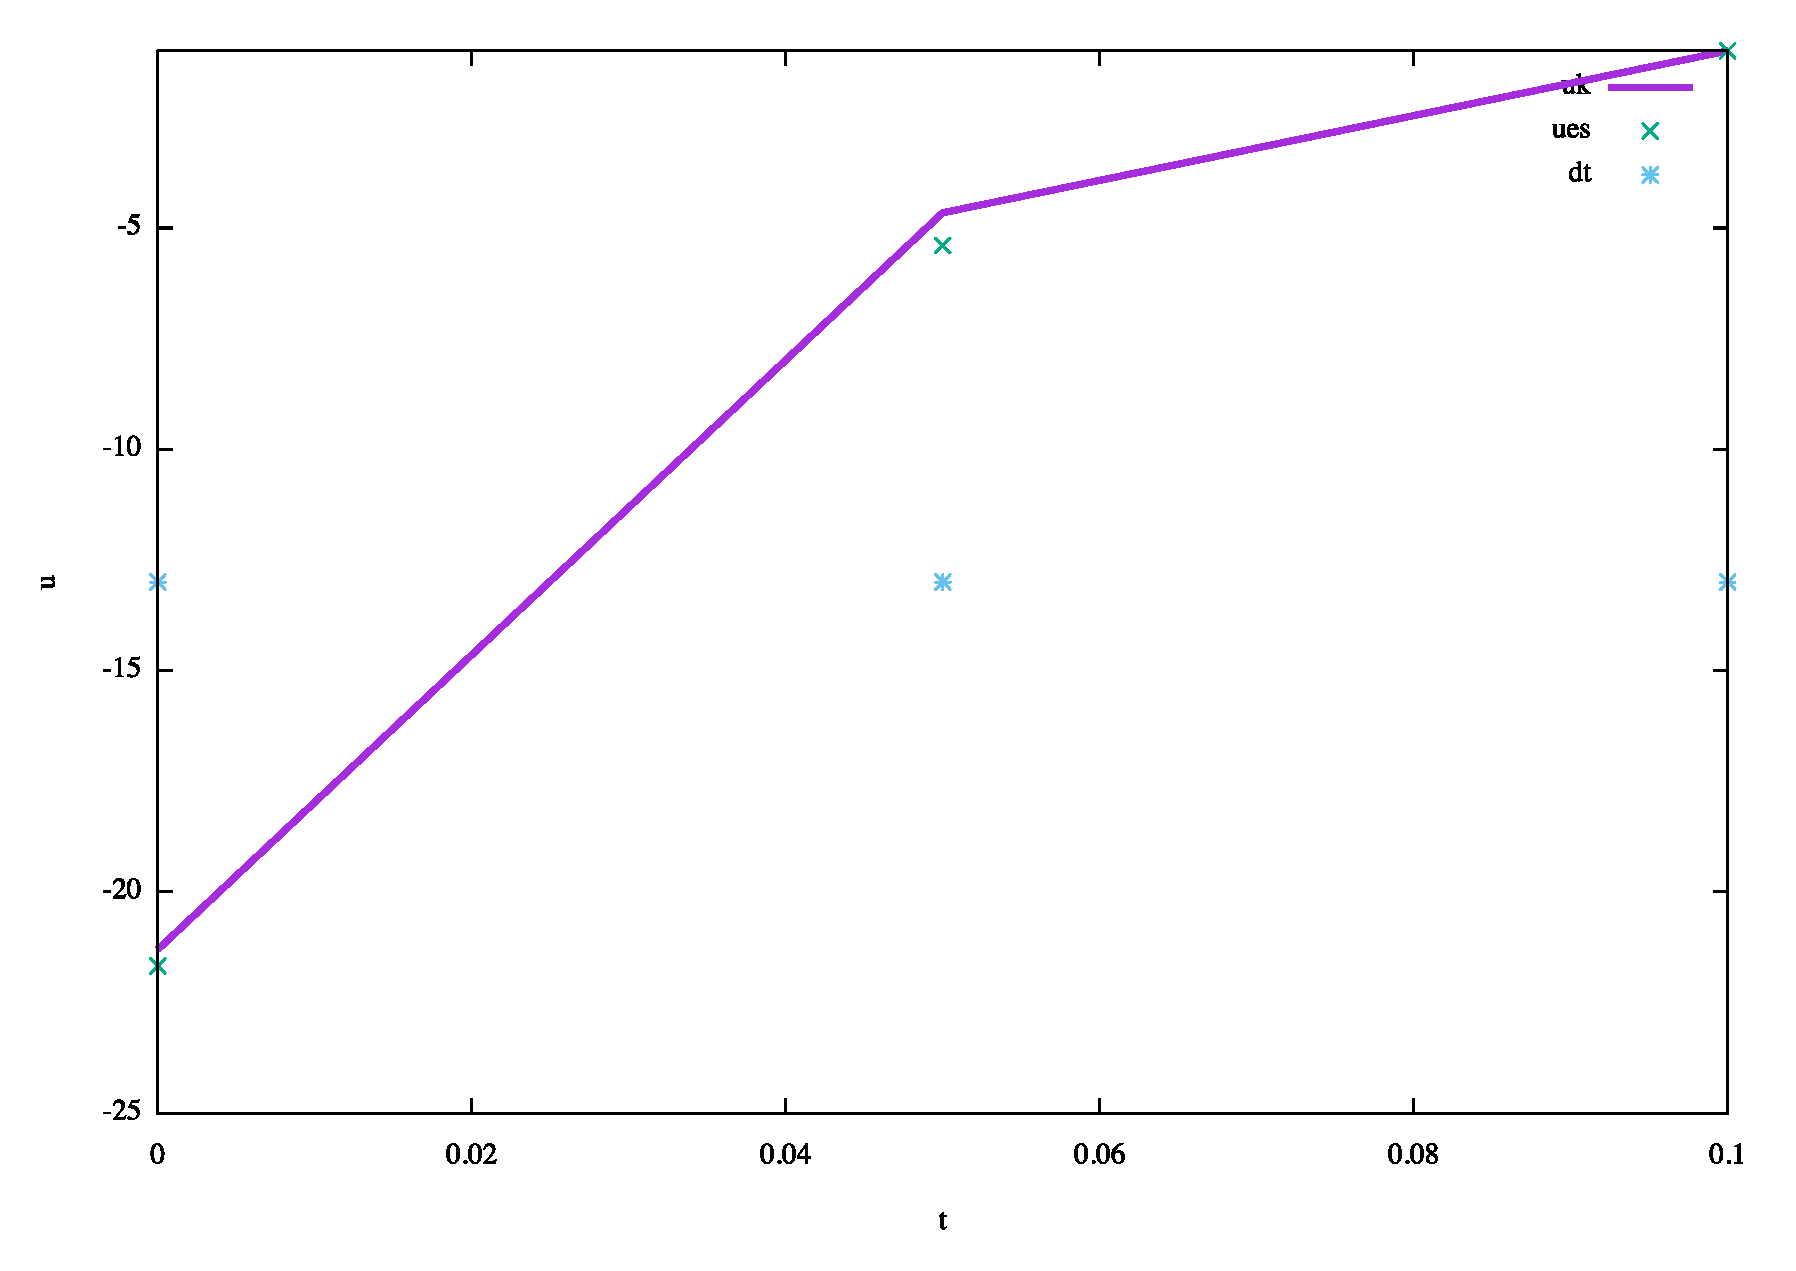
\includegraphics[width=0.3\linewidth]{img/cap6/Imm_PF_01/ControlSol_N150_l1}}\qquad
\subfigure[\protect\url{l = 2}]%
{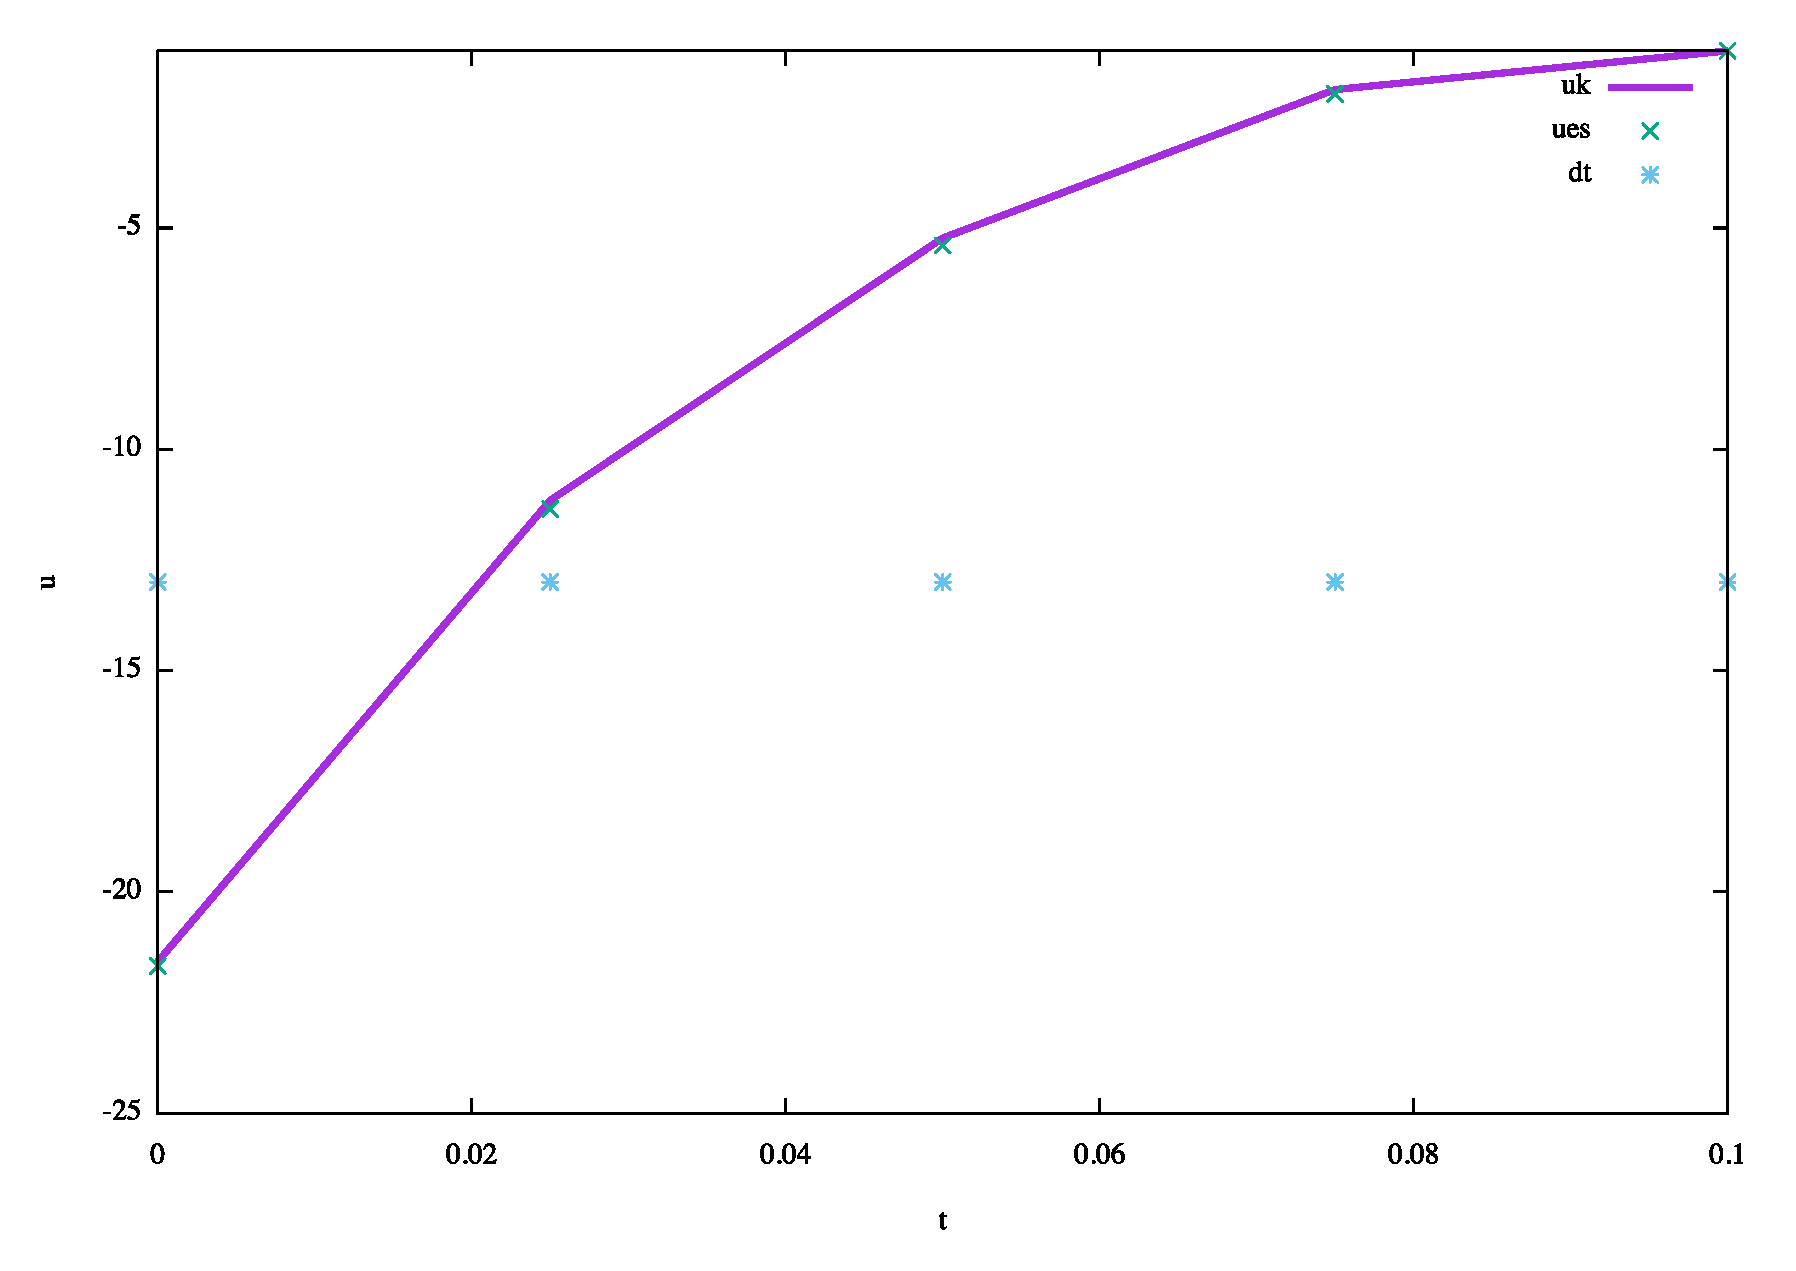
\includegraphics[width=0.3\linewidth]{img/cap6/Imm_PF_01/ControlSol_N150_l2}}\qquad
\subfigure[\protect\url{l = 3}]%
{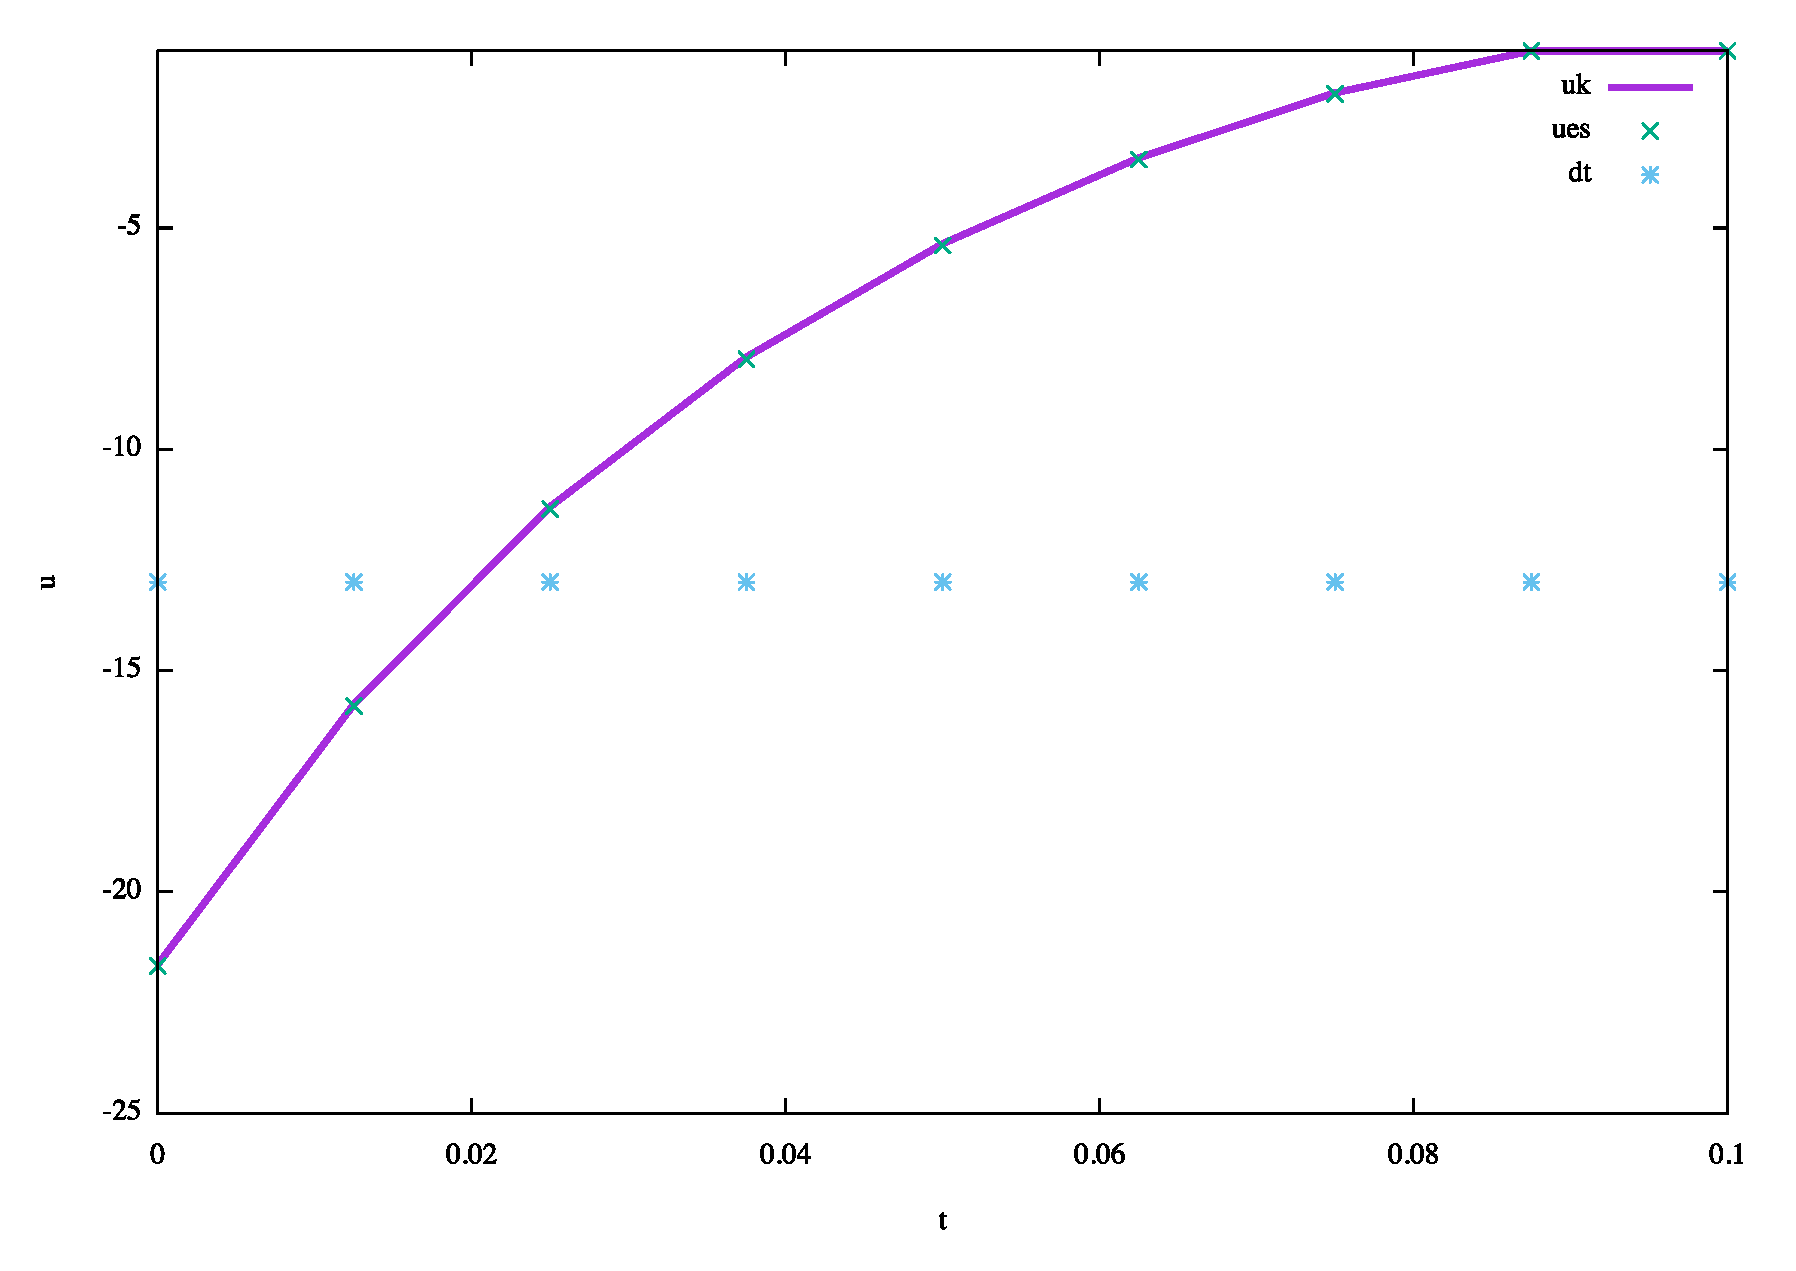
\includegraphics[width=0.3\linewidth]{img/cap6/Imm_PF_01/ControlSol_N150_l3}}\qquad
\subfigure[\protect\url{l = 4}]%
{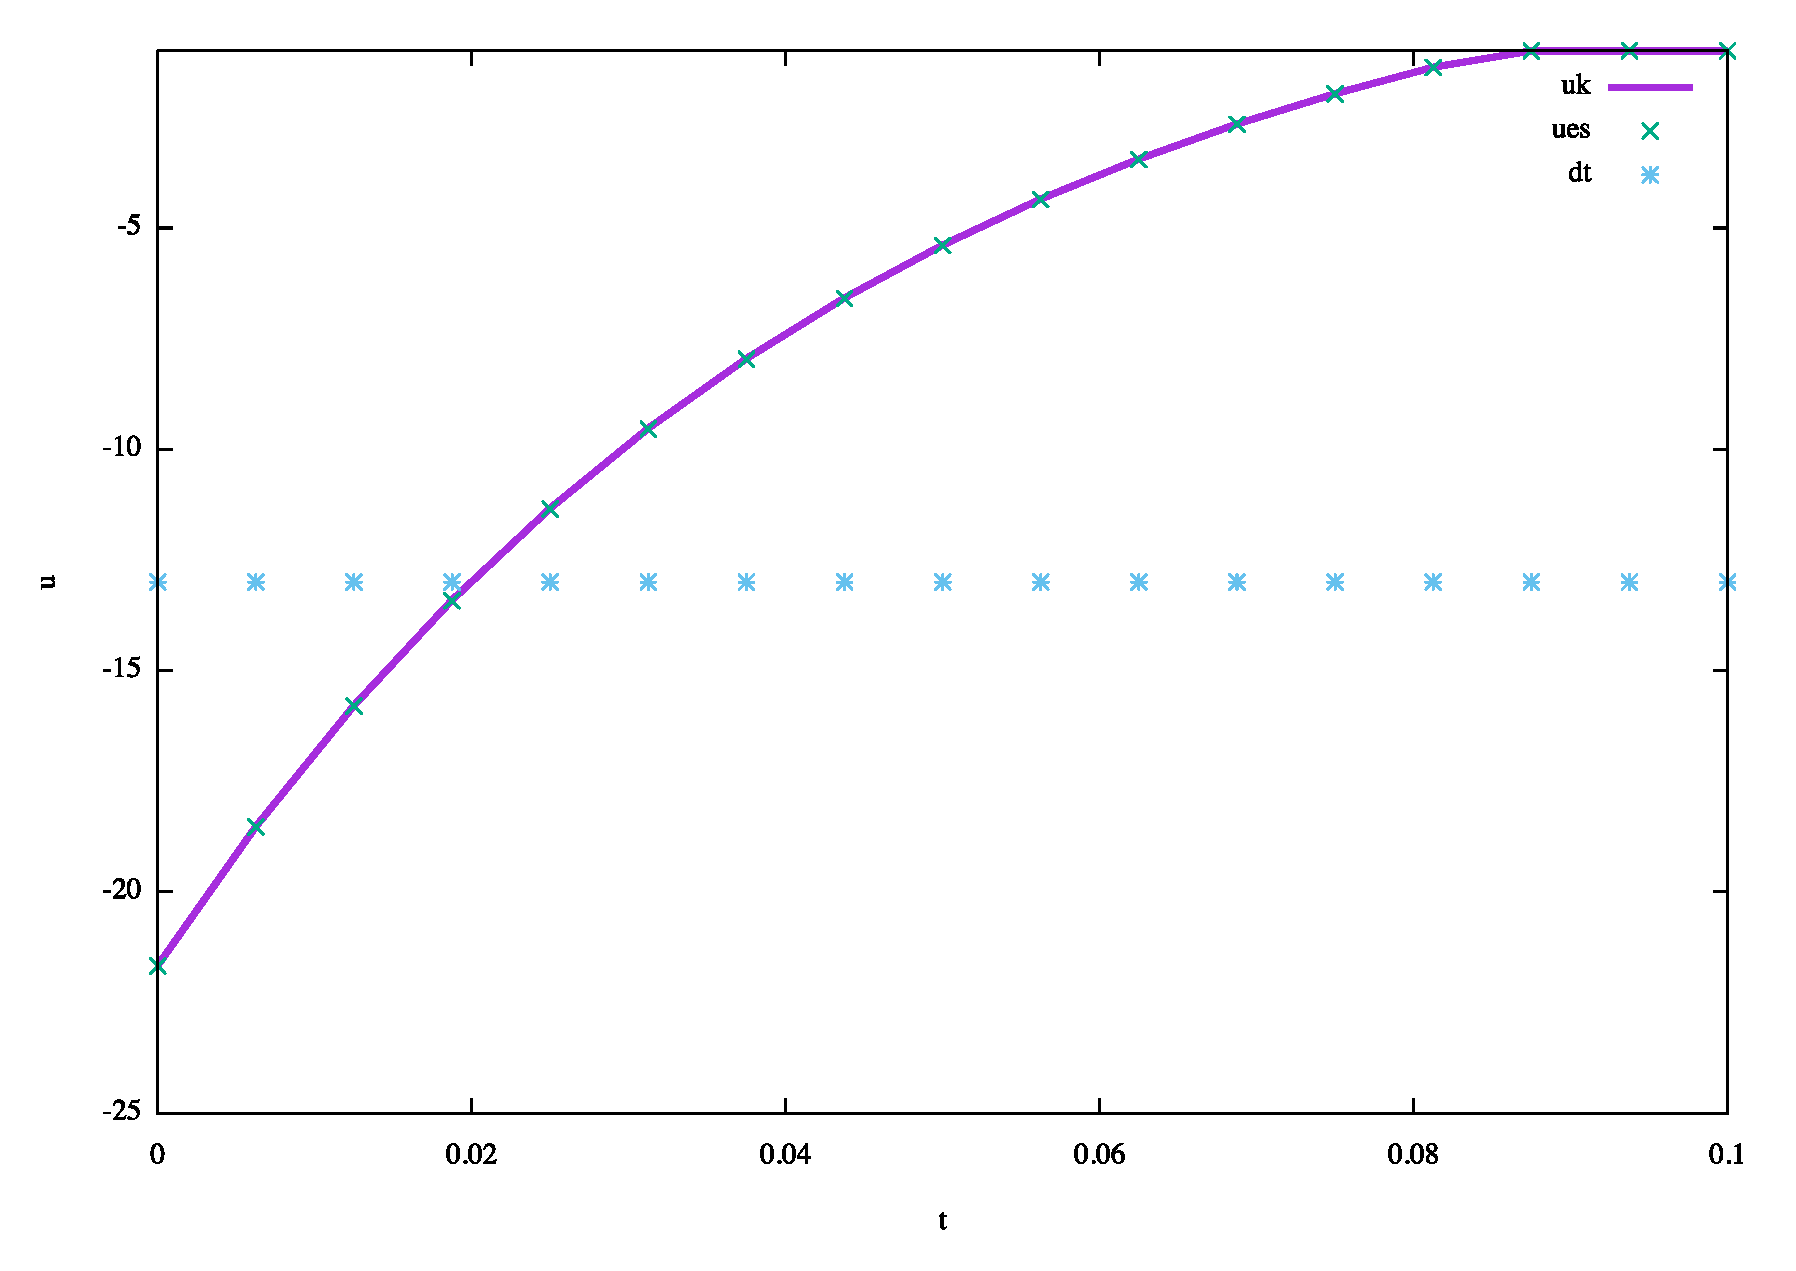
\includegraphics[width=0.3\linewidth]{img/cap6/Imm_PF_01/ControlSol_N150_l4}}\qquad
\subfigure[\protect\url{l = 5}]%
{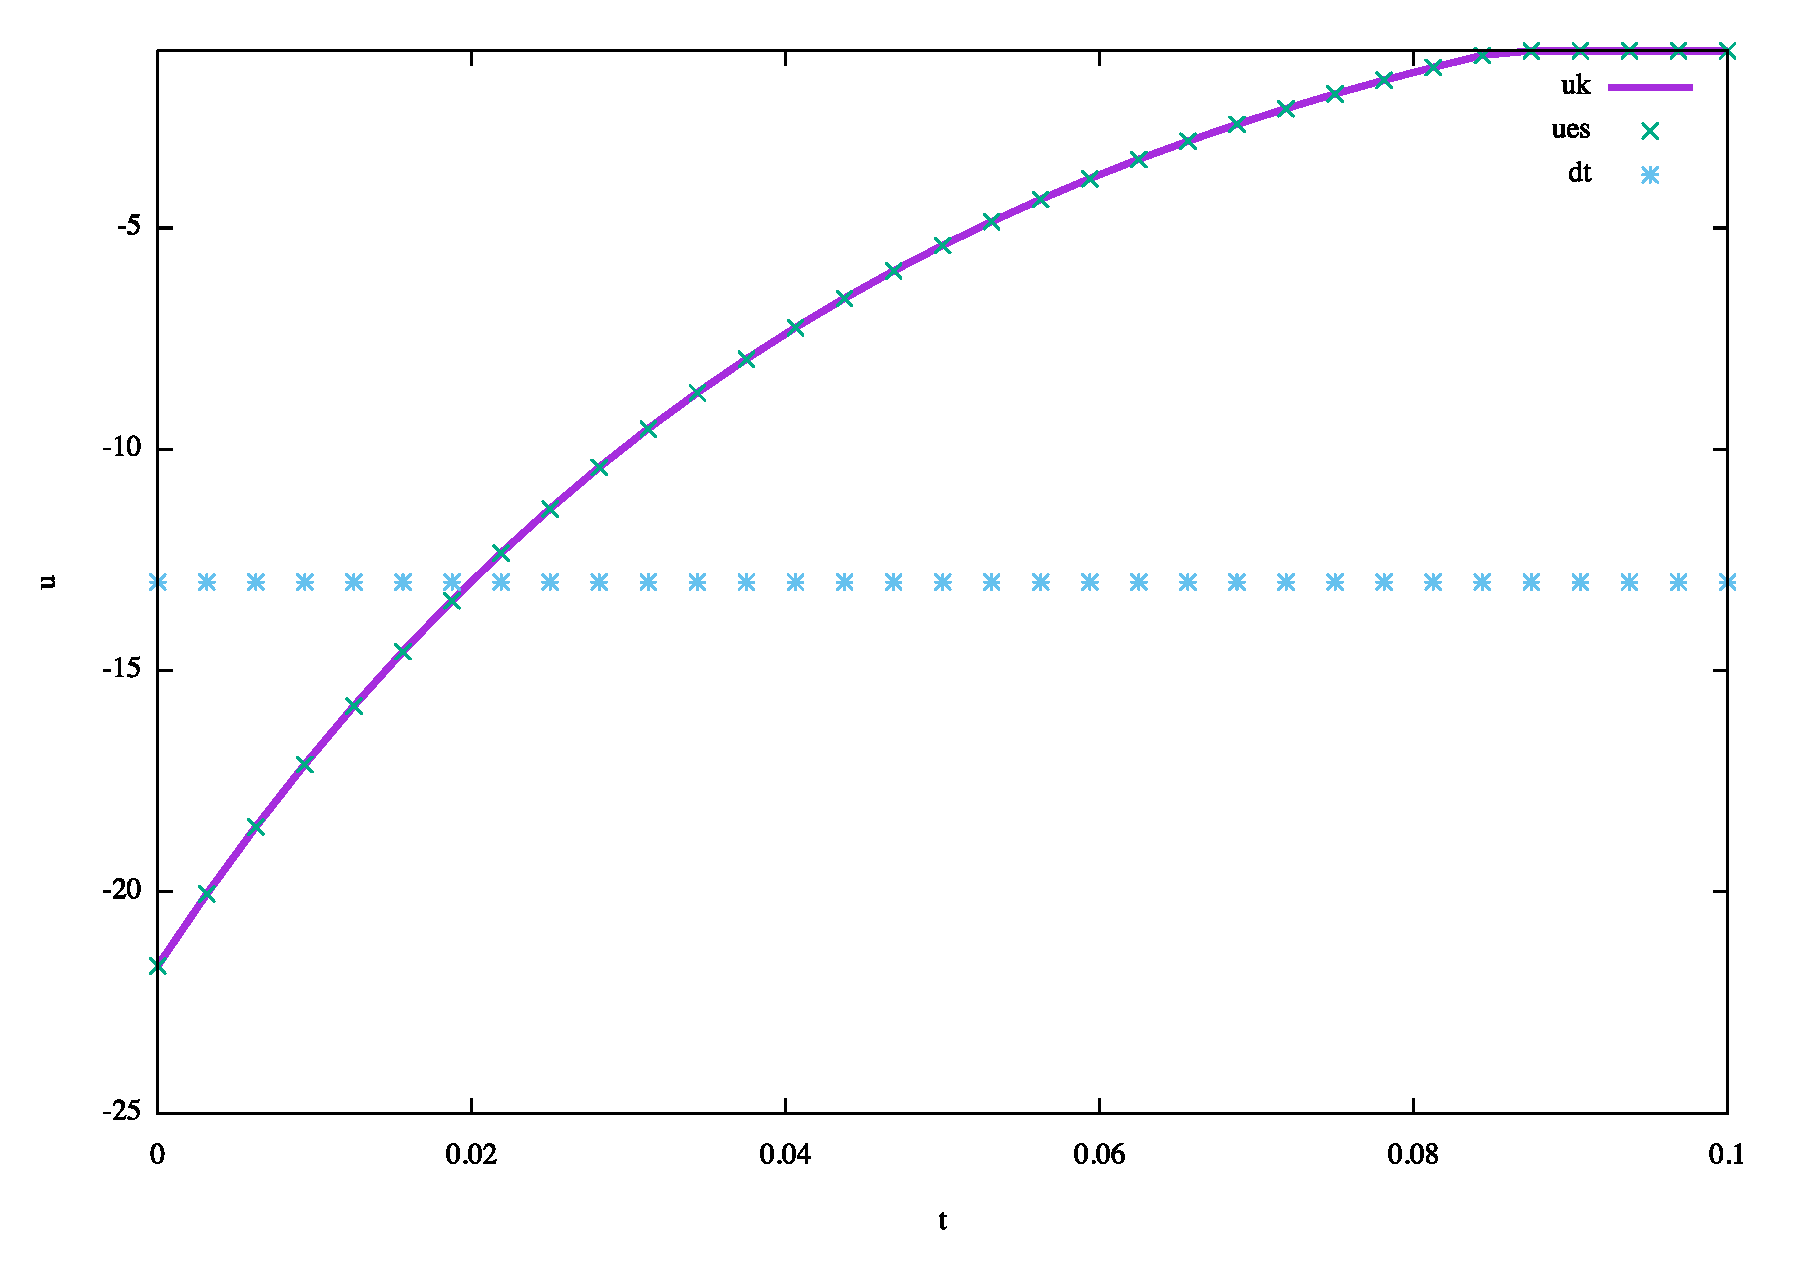
\includegraphics[width=0.3\linewidth]{img/cap6/Imm_PF_01/ControlSol_N150_l5}}\qquad
\subfigure[\protect\url{l = 6}]%
{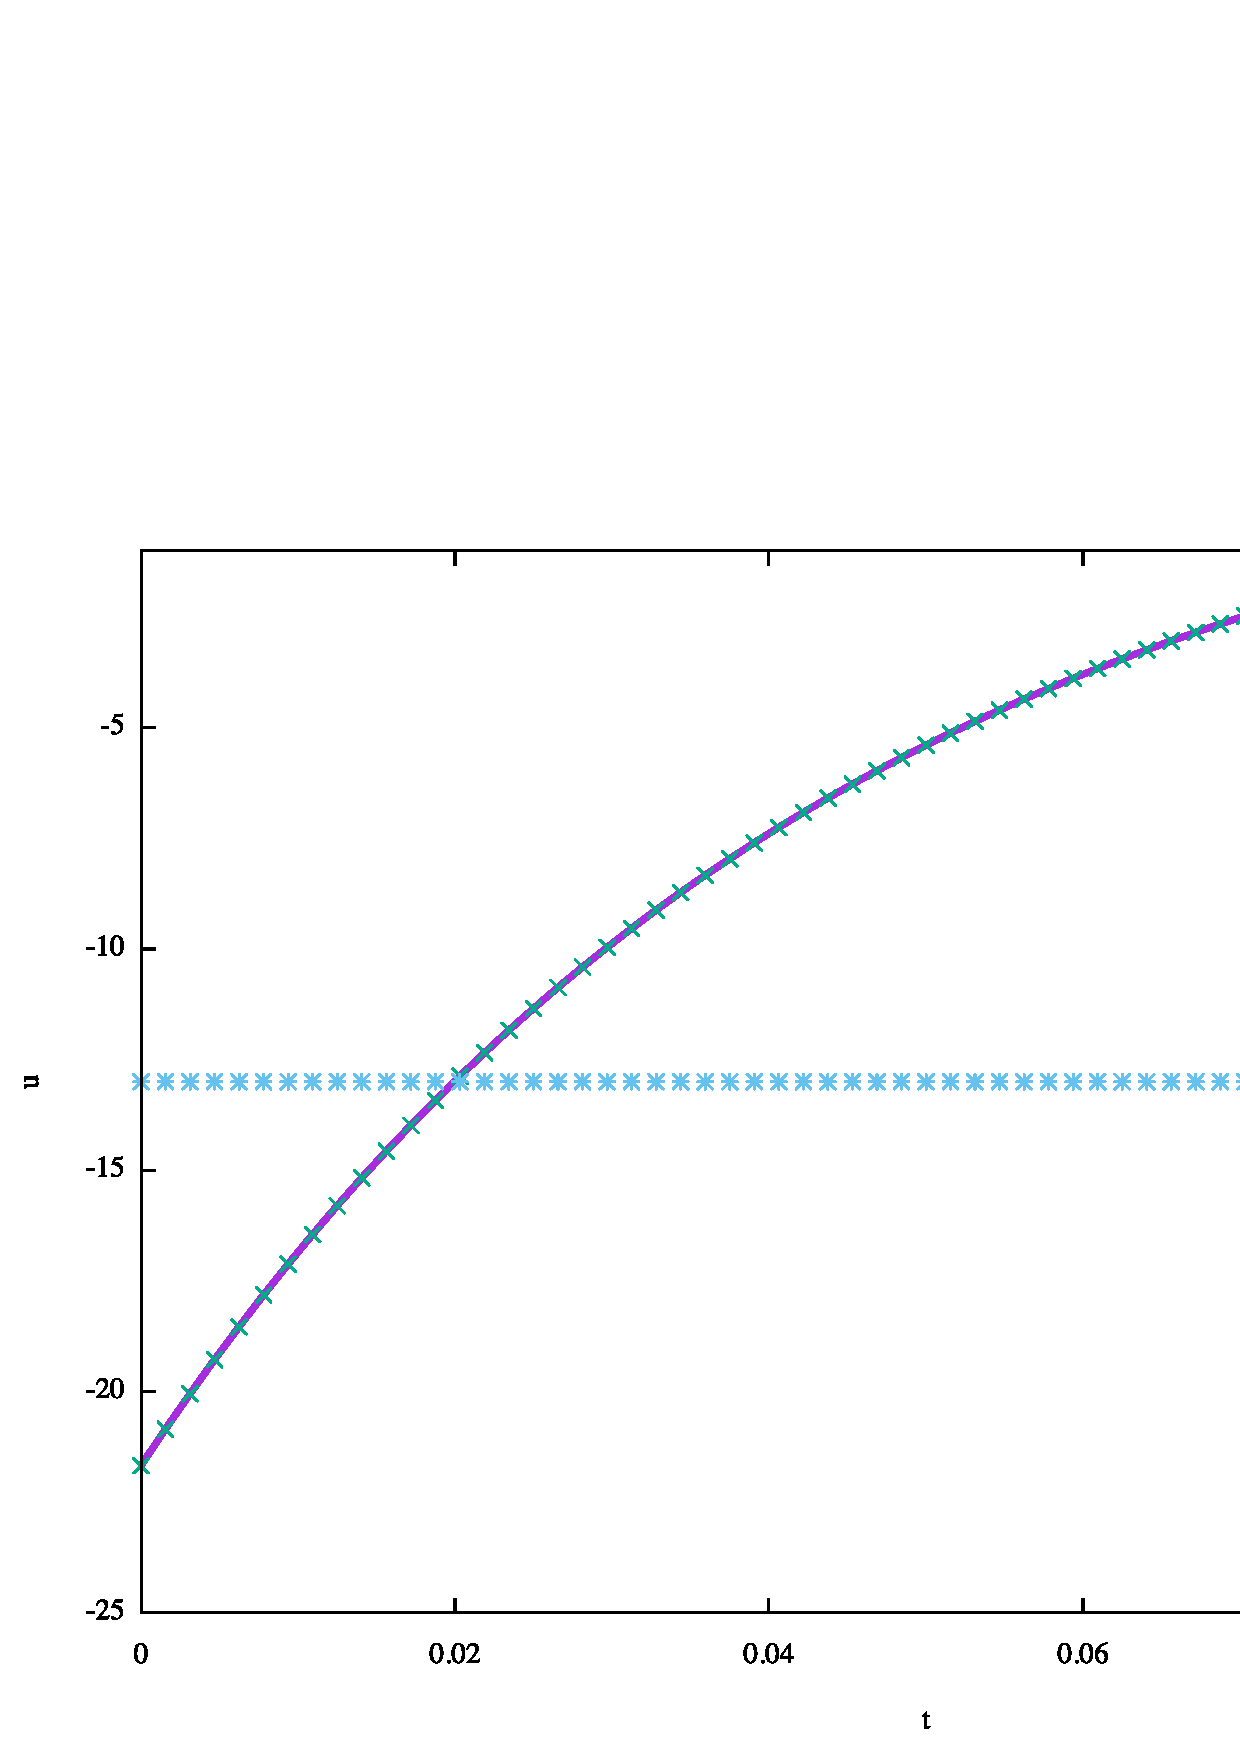
\includegraphics[width=0.3\linewidth]{img/cap6/Imm_PF_01/ControlSol_N150_l6}}
\label{fig:501}
\end{figure}

\end{frame}



\begin{frame}
\frametitle{Test Case 01 Punto fisso}
\begin{table}
\caption{Punto fisso per Test case 01: errori e EOC }
\label{puntofissoI}
\centering

\begin{tabular}{cllll}
\toprule
{l}           &  {$ \norma{\bar{u}-u_{kh}}_{L^2(L^2)} $} &  {$ \norma{\bar{y}-y_{kh}}_{L^2(L^2)} $} &  {$ EOC_u $} &  {$ EOC_y $} \\
\midrule
1            &  0.31667 &  0.981285 &  {$-$} &  {$-$} \\
2            &  0.0835064 &  0.496296 &  2.60937 &  1.33449 \\
3            &  0.0209608 &  0.248822 &  2.35165 &  1.17464 \\
4            &  0.00500916 &  0.124494 &  2.25065 &  1.08882 \\
5            &  0.00109219  &  0.0622586 &  2.29624 &  1.04473 \\
6            &  0.000497644 &  0.0311327 &  1.15957 &  1.02236 \\
\bottomrule
\end{tabular}              
\end{table}

\end{frame}

\begin{frame}
\frametitle{Test Case 01 Punto fisso}

\begin{table}
\caption{Punto fisso per Test case 01: errori e EOC }
\label{puntofissoIbis}
\centering

\begin{tabular}{cllll}
\toprule
{l}           &  {$ \norma{\bar{y}-\pi_{P^*_k}y_{kh}}_{L^2(L^2)} $} &  {$ \norma{\bar{p}-p_{kh}}_{L^2(L^2)} $} &  {$ EOC_{\pi y} $} &  {$ EOC_p $} \\
\midrule
1            &  0.520894 &  0.00660747 &  {$-$} &  {$-$} \\
2            &  0.15134 &  0.00173155 &  2.41965 &  2.6216 \\
3            &  0.0393476 &  0.00043334 &  2.29181 &  2.35673 \\
4            &  0.00970087 &  0.000103613 &  2.20164 &  2.24982 \\
5            &  0.00221619 &  0.000022824 &  2.2259 &  2.28078 \\
6            &  0.000432024 &  0.000010724 &  2.41203 &  1.11429 \\
\bottomrule
\end{tabular}              
\end{table}

\end{frame}

\begin{frame}
\frametitle{Test Case 01 Semi-Newton}


\end{frame}

\section{Conclusioni e Lavori Futuri}
\begin{frame}




\end{frame}

\end{document}